\documentclass{beamer}
%
% Choose how your presentation looks.
%
% For more themes, color themes and font themes, see:
% http://deic.uab.es/~iblanes/beamer_gallery/index_by_theme.html
%
\mode<presentation>
{
  \usetheme{default}      % or try Darmstadt, Madrid, Warsaw, ...
  \usecolortheme{default} % or try albatross, beaver, crane, ...
  \usefonttheme{serif}  % or try serif, structurebold, ...
  \setbeamertemplate{navigation symbols}{}
  \setbeamertemplate{caption}[numbered]
} 

\usepackage[english]{babel}
\usepackage[utf8x]{inputenc}
\usepackage[font=scriptsize,labelfont=bf]{caption}

\title[APC 524 Design Review]{Tabulation of Chemical Source Terms for Turbulent Combustion Simulations}
\author{Emmet Cleary \\
Daniel Floryan \\
Jeffry Lew \\
Bruce Perry \\
Emre Turkoz} 
\date{January 8, 2014}

\begin{document}

\begin{frame}
  \titlepage
\end{frame}

% Uncomment these lines for an automatically generated outline.
%\begin{frame}{Outline}
%  \tableofcontents
%\end{frame}

\section{Introduction}
\begin{frame}{Introduction}
\begin{figure}
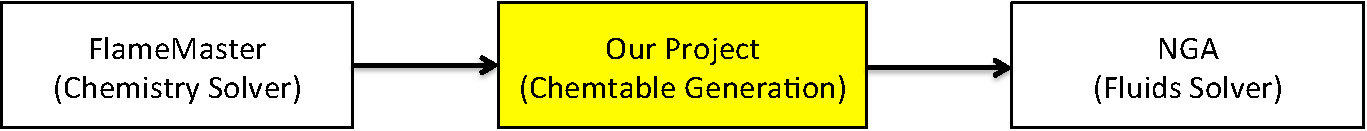
\includegraphics[width=\textwidth]{scope.pdf}
\end{figure}
\vskip 5mm
Key Capabilities:
\begin{itemize}
\item Sorting
\item Monotonicity checking
\item Convolution
\item Interpolation
\end{itemize}
\vspace{12pt}
SWIG will be used to interface C++ and Python.\\
Git will be used for version control.\\
DOxygen will be used for documentation.
\end{frame}


%%%%%%%%%%%%%%%%%%%%%%%%%%%%%%%%%%%%%%%%%%%%%%%%%%%%%%%%%%%%%%%%%%%%%%%%%%%%%%%%
%%%%%%%%%%%%%%%%%%%%%%%%%%%%%%%%%%%%%%%%%%%%%%%%%%%%%%%%%%%%%%%%%%%%%%%%%%%%%%%%
\section{Flowcharts}
%%%%%%%%%%%%%%%%%%%%%%%%%%%%%%%%%%%%%%%%%%%%%%%%%%%%%%%%%%%%%%%%%%%%%%%%%%%%%%%%
%%%%%%%%%%%%%%%%%%%%%%%%%%%%%%%%%%%%%%%%%%%%%%%%%%%%%%%%%%%%%%%%%%%%%%%%%%%%%%%%
\subsection{Progress Variable}
\begin{frame}{Progress Variable}
\begin{figure}
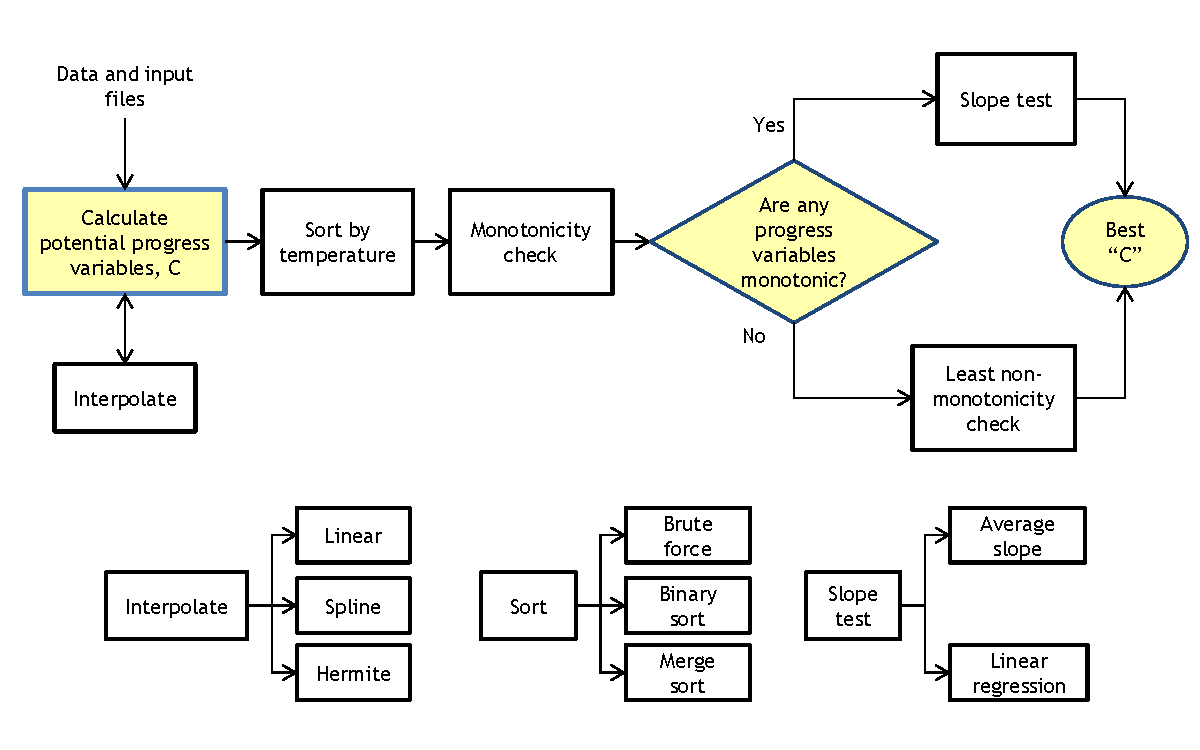
\includegraphics[width=\textwidth]{diagram_1_shortened_v1.pdf}
\end{figure}
\end{frame}

%%%%%%%%%%%%%%%%%%%%%%%%%%%%%%%%%%%%%%%%%%%%%%%%%%%%%%%%%%%%%%%%%%%%%%%%%%%%%%%%
\subsection{Table Generation}
\begin{frame}{Table Generation}
\begin{figure}
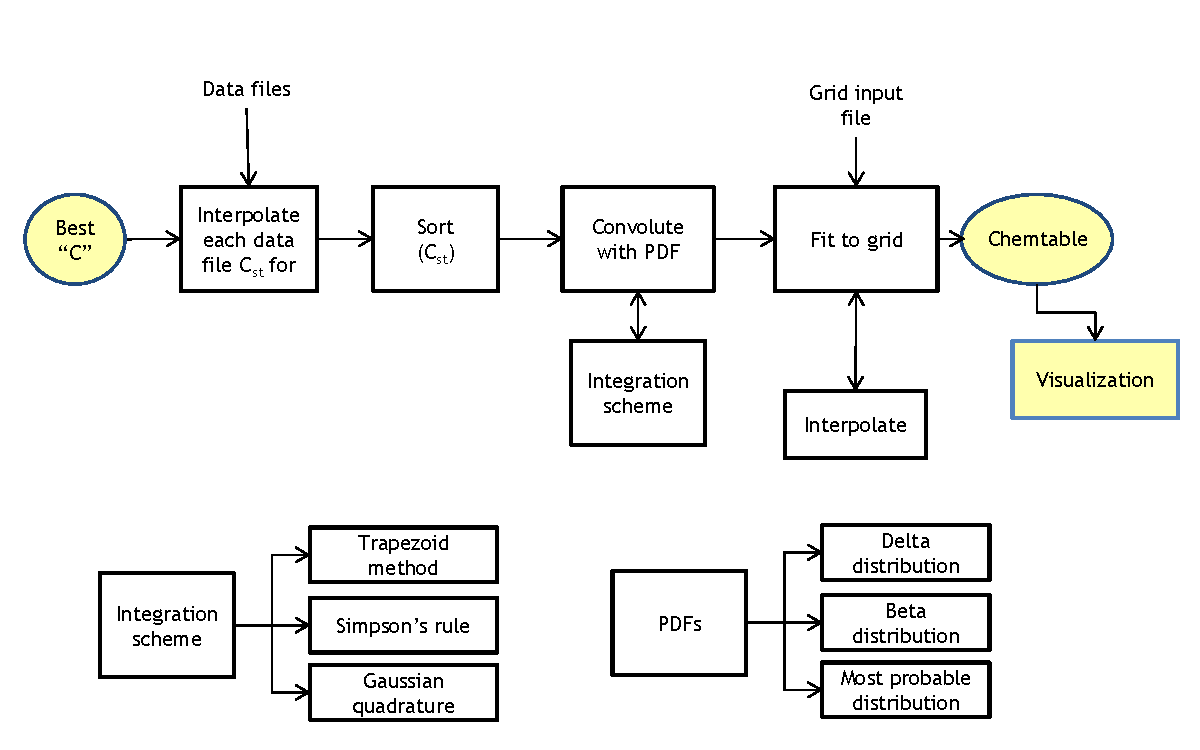
\includegraphics[width=\textwidth]{diagram_2_shortened_v1.pdf}
\end{figure}
\end{frame}


%%%%%%%%%%%%%%%%%%%%%%%%%%%%%%%%%%%%%%%%%%%%%%%%%%%%%%%%%%%%%%%%%%%%%%%%%%%%%%%%
%%%%%%%%%%%%%%%%%%%%%%%%%%%%%%%%%%%%%%%%%%%%%%%%%%%%%%%%%%%%%%%%%%%%%%%%%%%%%%%%
\section{Modules}
%%%%%%%%%%%%%%%%%%%%%%%%%%%%%%%%%%%%%%%%%%%%%%%%%%%%%%%%%%%%%%%%%%%%%%%%%%%%%%%%
%%%%%%%%%%%%%%%%%%%%%%%%%%%%%%%%%%%%%%%%%%%%%%%%%%%%%%%%%%%%%%%%%%%%%%%%%%%%%%%%
\subsection{Python: User Interface}
\begin{frame}{Python: User Interface}
\end{frame}

%%%%%%%%%%%%%%%%%%%%%%%%%%%%%%%%%%%%%%%%%%%%%%%%%%%%%%%%%%%%%%%%%%%%%%%%%%%%%%%%
%\subsection{Modules: Matrix/Matrix3D/Matrix4D}
%\begin{frame}{Modules: Matrix/Matrix3D/Matrix4D}
%Matrix.h/.i, Matrix3D.h/.i, Matrix4d.h/.i
%\begin{itemize}
%\item Matrix.cc
%\item Matrix3D.cc
%\item Matrix4D.cc
%\end{itemize}

%\vspace{10pt}
%Constructors:
%\begin{itemize}
%\item Matrix(int dim1, int dim2)
%\item Matrix3D(int dim1, int dim2, int dim3)
%\item Matrix4D(int dim1, int dim2, int dim3, int dim4)
%\end{itemize}

%\end{frame}

%%%%%%%%%%%%%%%%%%%%%%%%%%%%%%%%%%%%%%%%%%%%%%%%%%%%%%%%%%%%%%%%%%%%%%%%%%%%%%%%
\subsection{Modules: Sorting}
\begin{frame}{Modules: Sorting}
\end{frame}

%%%%%%%%%%%%%%%%%%%%%%%%%%%%%%%%%%%%%%%%%%%%%%%%%%%%%%%%%%%%%%%%%%%%%%%%%%%%%%%%
\subsection{Modules: Interpolate}
\begin{frame}{Modules: Interpolate}
\end{frame}

%%%%%%%%%%%%%%%%%%%%%%%%%%%%%%%%%%%%%%%%%%%%%%%%%%%%%%%%%%%%%%%%%%%%%%%%%%%%%%%%
\subsection{Modules: MonoCheck}
\begin{frame}{Modules: MonoCheck}
\end{frame}

%%%%%%%%%%%%%%%%%%%%%%%%%%%%%%%%%%%%%%%%%%%%%%%%%%%%%%%%%%%%%%%%%%%%%%%%%%%%%%%%
\subsection{Modules: MaxSlope/LeastNonMono}
\begin{frame}{Modules: MaxSlope/LeastNonMono}
\end{frame}

%%%%%%%%%%%%%%%%%%%%%%%%%%%%%%%%%%%%%%%%%%%%%%%%%%%%%%%%%%%%%%%%%%%%%%%%%%%%%%%%
\subsection{Modules: PDF}
\begin{frame}{Modules: PDF}
PDF.h/.i
\begin{itemize}
\item deltaPDF.h/.cc
\item betaPDF.h/.cc
\end{itemize}

%\vspace{10pt}
Constructors:
\begin{itemize}
\item DeltaPDF(const double *Mean)
\item BetaPDF(const double *Mean, const double *Variance)
\end{itemize}

%\vspace{10pt}
Virtual Functions:
\begin{itemize}
\item int valPDF(const double *Z, const int ZPoints, \\Matrix3D *pdfValues)
\end{itemize}

%\vspace{10pt}
Tests:
\begin{itemize}
\item Delta PDF: various means
\item Beta PDF: zero variance (Delta PDF), symmetric/skewed distributions, infinite boundaries
\end{itemize}
\end{frame}


%%%%%%%%%%%%%%%%%%%%%%%%%%%%%%%%%%%%%%%%%%%%%%%%%%%%%%%%%%%%%%%%%%%%%%%%%%%%%%%%
\subsection{Module: Integrator}
\begin{frame}{Modules: Integrator}
Integrator.h/.i
\begin{itemize}
\item Trapz.h/.cc
\item Simpson.h/.cc
\item GLQuad.h/.cc
\end{itemize}

Constructors
\begin{itemize}
\item Trapz()
\item Simpson()
\item GLQuad(int Nodes)
\end{itemize}

Virtual Functions:
\begin{itemize}
\item double integrate(const double *integrand, const double *Z, const int ZPoints)
\end{itemize}

Tests:
\begin{itemize}
\item Various functions
\end{itemize}
\end{frame}

%%%%%%%%%%%%%%%%%%%%%%%%%%%%%%%%%%%%%%%%%%%%%%%%%%%%%%%%%%%%%%%%%%%%%%%%%%%%%%%%
\subsection{Modules: Convolute}
\begin{frame}{Modules: Convolute}
Convolute.h/.i
\begin{itemize}
\item Convolute.h/.cc
\end{itemize}

Functions:
\begin{itemize}
\item int convVal(double *Z, double *data, \\Matrix3D *pdfValues, Matrix *return, Integrator *intgr)
\end{itemize}

Tests:
\begin{itemize}
\item Convolute with 1 using all PDFs/Integrators
\end{itemize}
\end{frame}

%%%%%%%%%%%%%%%%%%%%%%%%%%%%%%%%%%%%%%%%%%%%%%%%%%%%%%%%%%%%%%%%%%%%%%%%%%%%%%%%
\subsection{Modules: FitToGrid}
\begin{frame}{Modules: FitToGrid}
\end{frame}

% DEMO

%%%%%%%%%%%%%%%%%%%%%%%%%%%%%%%%%%%%%%%%%%%%%%%%%%%%%%%%%%%%%%%%%%%%%%%%%%%%%%%%
\subsection{Profiling}
\begin{frame}{Profiling}
\end{frame}












\end{document}
